\section{Profitability of partial outsourcing}
\label{sec:partial-outsourcing}

The pool operator may still have opportunity to partially outsource mining.
$\mathsf{VRFHash}$ consists of three steps: $h \gets H_1(\alpha)$, $\gamma \gets h^{sk}$ and $\beta \gets H_2(\gamma)$.
The non-outsourceability is from the second step $\gamma = h^{sk}$, as it requires the knowledge of the pool operator's secret key $sk$.
The pool operator can outsource the first step $h = H_1(\alpha)$ by distributing different $\alpha$s to miners, and also the last step $\beta = H_2(\gamma)$ by distributing different $\gamma$s to miners.

However, such partial outsourcing is very inefficient and unprofitable compared to outsourcing in hash-based mining, due to the computing and I/O overhead.
In this section, we show that partial outsourcing in VRF-based mining is unprofitable as it's computation-intensive and I/O intensive.
We also show that making VRF fast can make VRF-based mining even more costly.

\subsection{Partial outsourcing in VRF-based mining}

\begin{figure}[]
    \centering
    \begin{msc}{}
        \setlength{\envinstdist}{2.5cm}

        \setlength{\instdist}{4cm}
        \setlength{\instwidth}{1.5cm}
        
        \declinst{pool}{}{Pool}
        \declinst{miner}{}{Miner}

        \action*{\parbox{4.5cm}{
            Get block template $t$\\
            Get pool mining difficulty $PT$\\
            Get nonce interval $[n_1, n_m]$
        }}{pool}

        \nextlevel[4]
        \mess{$n_1, n_m, t$}{pool}{miner}

        \nextlevel
        \action*{\parbox{3cm}{
            For all $k \in [1, m]$\\
            \tab $h_k \gets H_1(t||n_k)$
        }}{miner}

        \nextlevel[3]
        \mess{$h_1, h_2, \dots, h_m$}{miner}{pool}

        \nextlevel
        \action*{\parbox{3.8cm}{
            For all $k \in [1, m]$\\
            \tab Check if $h_k = H(t||n_k)$\\
            \tab $\gamma_k \gets {h_k}^{sk}$
        }}{pool}

        \nextlevel[5]
        \mess{$\gamma_1, \gamma_2, \dots, \gamma_m, PT$}{pool}{miner}

        \nextlevel
        \action*{\parbox{3.5cm}{
            $\Gamma \gets []$\\
            For all $k \in [1, m]$\\
            \tab $out_k \gets H_2(\gamma_k)$\\
            \tab if $out_k < PT$\\
            \tab\tab Append $\gamma_k$ to $\Gamma$
        }}{miner}

        \nextlevel[6]
        \mess{$\Gamma$}{miner}{pool}

        \nextlevel
        \action*{\parbox{4.5cm}{
            (Optional) For all $\gamma_j \in \Gamma$\\
            \tab Check if $\gamma_j \in (\gamma_1, \dots, \gamma_m)$\\
            \tab if $H_2(\gamma_j) < PT$\\
            \tab\tab Mined a share 
        }}{pool}

        \nextlevel[5]

    \end{msc}
    \caption{Partial outsourcing in VRF-based mining.}
    \label{fig:outsource-vrf}
\end{figure}


Figure~\ref{fig:outsource-vrf} describe the process of outsourcing $H_1(\cdot)$ and $H_2(\cdot)$.
In VRF-based mining, the second step $h^{sk}$ is non-outsourceable, but the pool operator can outsource $H_1(\cdot)$ or $H_2(\cdot)$ interactively.

To outsource $H_1(\cdot)$, the pool operator generates a search interval $[n_1, n_m]$ of nonces, then sends the interval and the block template $t$ to a miner.
After that, the miner computes $H_1(\cdot)$ with each nonce in $[n_1, n_m]$ as input, then sends back all $H_1(\cdot)$ hashes to the pool operator.
If the pool operator does not trust miners (which reflects to the real world), he will verify these $H_1(\cdot)$ hashes before the second step i.e., multiplying each hash with his secret key $sk$.

After the second step, the pool operator obtains a series of $(\gamma_1, \gamma_2, \dots, \gamma_m)$, and he can outsource $H_2(\cdot)$ as follows.
The pool operator first sends these $\gamma$s as well as the pool difficulty $PoolTarget$ to the miner.
Then, the miner calculates $H_2(\cdot)$ hashes of these $\gamma$s, compare the hashes with $PoolTarget$, and sends back $\gamma$s that satisfy the difficulty (denoted as $\Gamma$).
Similarly, the pool operator optionally verifies the correctness of each of $\Gamma$, and accumulates the mined shares to the miner's total contribution.


\subsection{The cost of verifying hashes from miners}

The first obstacle of partial outsourcing is verifying hashes from miners.
If the pool operator does not trust miners, he should verify both $H_1(\cdot)$ and $H_2(\cdot)$ hashes from miners.
For outsourcing $H_1(\cdot)$, the pool operator should verify all of $h_1, h_2, \dots, h_m$.
For outsourcing $H_2(\cdot)$, The pool operator should verify $\sigma$s satisfying $PoolTarget$.
This introduces significant overhead, which is equivalent to mining by the pool operator himself.
Thus, partial outsourcing unprofitable.


\subsection{Partial outsourcing is I/O intensive}

To workaround the verification overhead, the pool operator and the miners should trust each other.
The pool operator and miners are still possible to collaborate, as pooled mining is beneficial for them.
For the pool operator, he can earn some fees from the miners.
For the miners, they can stabilise their revenue from mining.

However, even if they trust each other, partial outsourcing can still be unprofitable.
VRF-based mining can be extremely I/O intensive, while the pool operator's server suffers from limited bandwidth.
To outsource a single $H_1(\cdot)$ in VRF-based mining, the pool operator should at least receive a $H_1(\cdot)$ hash from the miner
To outsource a single $H_2(\cdot)$, the pool operator should at least send a $\sigma$ to the miner.
% hash based mining does not suffer from this problem
Hash-based mining does not suffer from this problem.
In hash-based mining, the pool operator only sends and receives constant-size data for each share.
By increasing the share difficulty, the pool operator will receive fewer shares and support more miners.

We model the maximum hashrate the pool operator can support as follows.
Consider a pool operator with bandwidth $BW$ (in bytes/s), and the pool operator can achieve optimal bandwidth utilisation on mining.
Assume the pool operator should transfer $N$ bytes per hash.
Thus, the maximum hashrate is

$$\text{Maximum hashrate} = \frac{BW}{N}$$

Either a $H_1(\cdot)$ hash and a $\gamma$ (a point on the elliptic curve) at least takes 32 bytes.
If outsourcing both $H_1(\cdot)$ and $H_2(\cdot)$, the maximum hashrate the pool operator can support is $\text{Maximum Hashrate} = \frac{BW}{64} (h/s)$.
If outsourcing only one of them, the maximum hashrate is $\text{Maximum Hashrate} = \frac{BW}{32} (h/s)$.

\begin{figure}[htp]
    \centering
    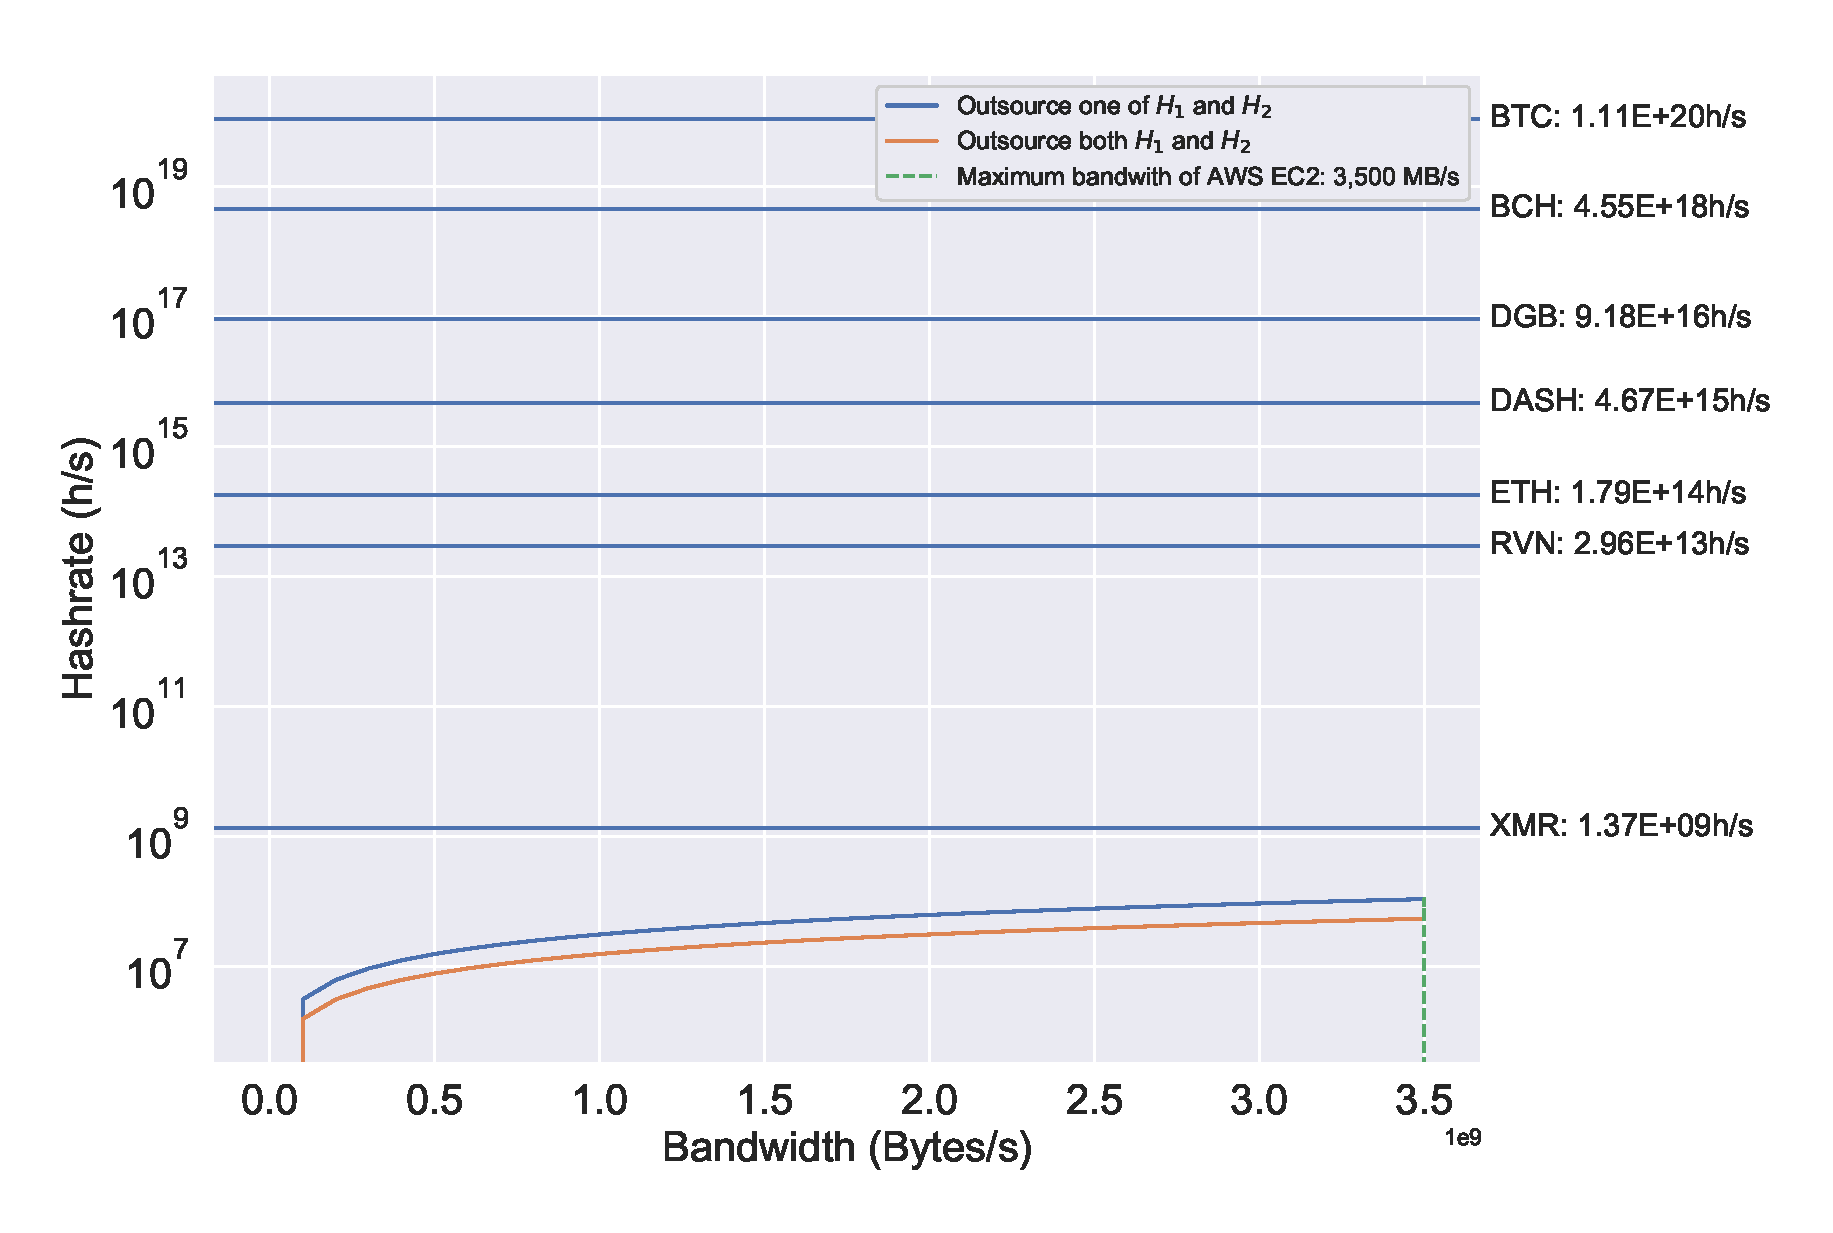
\includegraphics[width=\linewidth]{figs/max-hashrate.eps}
    \caption{Server bandwidth v.s. maximum hashrate.
    Data of server bandwidth and hashrate were fetched from \cite{aws} and \cite{coinwarz}.}
    \label{fig:max-hashrate}
\end{figure}

Figure~\ref{fig:max-hashrate} shows relationship between the pool operator's network bandwidth maximum and the maximum hashrate.
The result shows that, even a server with most bandwidth from AWS (I3EN Metal with 3,500 MB/s) can only support less than $\frac{1}{10}$ of Monero's total mining power.
Within those mainstream cryptocurrencies, Monero's hashrate is the least.
Even if the pool operator rents a cluster of I3EN Metal machines for more bandwidth, I3EN Metal is quite expensive (10.848 USD per hour), leading to high expense of maintaining a mining pool.
Therefore, partial outsourcing in VRF-based mining is costly and unrealistic.
By embedding lightweight mining algorithms in VRFs such as SHA256D, VRF-based mining can be maximally I/O-intensive.
